\documentclass[12pt]{report}
\usepackage[utf8]{inputenc}
\usepackage[russian]{babel}
%\usepackage[14pt]{extsizes}
\usepackage{listings}
\usepackage{amsmath}
\usepackage[justification=centering]{caption}

% Для листинга кода:
\lstset{ %
language=c,                 % выбор языка для подсветки (здесь это С)
basicstyle=\footnotesize\sffamily, % размер и начертание шрифта для подсветки кода
numbers=left,               % где поставить нумерацию строк (слева\справа)
numberstyle=\tiny,           % размер шрифта для номеров строк
stepnumber=1,                   % размер шага между двумя номерами строк
numbersep=5pt,                % как далеко отстоят номера строк от подсвечиваемого кода
showspaces=false,            % показывать или нет пробелы специальными отступами
showstringspaces=false,      % показывать или нет пробелы в строках
showtabs=false,             % показывать или нет табуляцию в строках
frame=single,              % рисовать рамку вокруг кода
tabsize=2,                 % размер табуляции по умолчанию равен 2 пробелам
captionpos=t,              % позиция заголовка вверху [t] или внизу [b] 
breaklines=true,           % автоматически переносить строки (да\нет)
breakatwhitespace=false, % переносить строки только если есть пробел
escapeinside={\#*}{*)}   % если нужно добавить комментарии в коде
}

\usepackage{hyperref}
\hypersetup{
    linktoc=all,     %set to all if you want both sections and subsections linked
    linkcolor=blue,  %choose some color if you want links to stand out
}

% Для измененных титулов глав:
\usepackage{titlesec, blindtext, color} % подключаем нужные пакеты
\definecolor{gray75}{gray}{0.75} % определяем цвет
\newcommand{\hsp}{\hspace{20pt}} % длина линии в 20pt
% titleformat определяет стиль
\titleformat{\chapter}[hang]{\Huge\bfseries}{\thechapter\hsp\textcolor{gray75}{|}\hsp}{0pt}{\Huge\bfseries}

% plot
\usepackage{pgfplots}
\usepackage{filecontents}
\usetikzlibrary{datavisualization}
\usetikzlibrary{datavisualization.formats.functions}

\begin{document}
\begin{titlepage}
	\fontsize{12pt}{12pt}\selectfont
	\noindent \begin{minipage}{0.15\textwidth}
		
\includegraphics[width=\linewidth]{inc/img/b_logo.jpg}
	\end{minipage}
	\noindent\begin{minipage}{0.9\textwidth}\centering
		\textbf{Министерство науки и высшего образования Российской Федерации}\\
		\textbf{Федеральное государственное бюджетное образовательное учреждение высшего образования}\\
		\textbf{«Московский государственный технический университет имени Н.Э.~Баумана}\\
		\textbf{(национальный исследовательский университет)»}\\
		\textbf{(МГТУ им. Н.Э.~Баумана)}
	\end{minipage}
	
	\noindent\rule{15cm}{3pt}
	\newline\newline
	\noindent ФАКУЛЬТЕТ \underline{~~~~~~~~~~~~~~~~«Информатика и системы управления»~~~~~~~~~~~~~~~~} \newline\newline
	\noindent КАФЕДРА \underline{«Программное обеспечение ЭВМ и информационные технологии»}\newline\newline\newline\newline\newline\newline\newline
	
	
	\begin{center}
		\Large\textbf{Отчет по лабораторной работе №7 по курсу "Анализ алгоритмов"}\newline
	\end{center}
	
	\noindent\textbf{Тема} \underline{Поиск в словаре}\newline\newline\newline
	\noindent\textbf{Студент} \underline{Якуба Д. В.}\newline\newline
	\noindent\textbf{Группа} \underline{ИУ7-53Б}\newline\newline
	\noindent\textbf{Оценка (баллы)} \underline{~~~~~~~~~~~~~~~~~~~}\newline\newline
	\noindent\textbf{Преподаватели} \underline{Волкова Л.Л., Строганов Ю.В.}\newline
	
	\begin{center}
		\vfill
		Москва~---~\the\year
		~г.
	\end{center}
\end{titlepage}

\setcounter{page}{2}

\tableofcontents

\newpage
\chapter*{Введение}
\addcontentsline{toc}{chapter}{Введение}
\section*{Цель лабораторной работы}
Реализация алгоритмов поиска по словарю: перебором, бинарным поиском и с применением частотного анализа.
\section*{Задачи лабораторной работы}
\begin{enumerate}
\item[1)] изучить алгоритм поиска по словарю полным перебором;
\item[2)] изучить алгоритм бинарного поиска по словарю;
\item[3)] изучить алгоритм поиска по словарю с применением частотного анализа;
\item[4)] протестировать реализованные алгоритмы;
\item[5)] провести анализ временных характеристик реализованных алгоритмов;
\item[6)] подготовить отчёт по проведенной работе.
\end{enumerate}

\chapter{Аналитическая часть}
В данном разделе описаны определение словаря как структуры данных, а также алгоритмы поиска по словарю.

\section{Словарь}
Словарь (ассоциативный массив)\cite{NIST} — это абстрактный тип данных, хранящий пары вида «(ключ, значение)» и поддерживающий операции добавления пары, а также поиска и удаления пары по ключу:
\begin{itemize}
\item $INSERT(\textit{ключ, значение}$;
\item $FIND(\textit{ключ})$;
\item $REMOVE(\textit{ключ})$.
\end{itemize}

Предполагается, что все ключи в словаре являются уникальными.

В паре $(\textit{ключ, значение})$ $\textit{значение}$ называется значением, ассоциированным с ключом.

Операция $FIND(\textit{ключ})$ возвращает значение, ассоциированное с заданным ключом, или некоторый специальный объект, означающий, что значения, ассоциированного с заданным ключом, нет. Две другие операции ничего не возвращают (за исключением, возможно, информации о том, успешно ли была выполнена данная операция).

\section{Алгоритм поиска по словарю полным перебором}
Алгоритм полного перебора \cite{AI} — это алгоритм разрешения математических задач, который можно отнести к классу способов нахождения решения рассмотрением всех возможных вариантов.

Для решения поставленной задачи поиска с использованием метода полного перебора потребуется последовательно просматривать каждую запись в словаре. В том случае, если у рассматриваемой пары ключ совпадает с искомым - алгоритм завершает свою работу, задача выполнена.

Трудоёмкость алгоритма зависит от того, присутствует ли искомый ключ в словаре, и, если присутствует - насколько он далеко от начала массива ключей.

При решении задачи возможно возникновение $(N + 1)$ случаев, где $N$ - это количество записей в словаре: ключ не найден и $N$ возможных случаев расположения ключа в словаре.

Лучшим случаем для рассматриваемого алгоритма будет факт того, что искомый ключ был обнаружен за одно сравнение (то есть ключ находится в начале словаря).

Худший случай наступает при следующих стечениях обстоятельств:
\begin{itemize}
\item элемент не был найден за $N$ сравнений;
\item ключ был обнаружен на последнем сравнении.
\end{itemize}

Пусть на старте алгоритм поиска затрачивает $k_0$ операций, а при каждом сравнении $k_1$ операций. Тогда в лучшем случае потребуется $k_0 + k_1$ операций; в случае, если ключ был найден на втором сравнении - потребуется $k_0 + 2k_1$ операций; в случае нахождения ключа на последней позиции или его отсутствия в словаре - потребуется $k_0 + Nk_1$ операций.

Средняя трудоёмкость алгоритма может быть рассчитана как математическое ожидание по формуле \ref{MX} ($\Omega$ - множество всех возможных исходов).

\label{MX}
\begin{multline}
        \sum\limits_{i \in \Omega} p_i \cdot f_i = (k_0 + k_1) \cdot \frac{1}{N + 1} + (k_0 + 2 \cdot k_1) \cdot \frac{1}{N+1} + (k_0 + 3 \cdot k_1) \cdot \frac{1}{N + 1} + \\+ (k_0 + Nk_1)\frac{1}{N + 1} + (k_0 + N \cdot k_1) \cdot \frac{1}{N + 1} = \\= k_0\frac{N+1}{N+1}+k_1+\frac{1 + 2 + \cdots + N + N}{N + 1} = k_0 + k_1 \cdot \left(\frac{N}{N + 1} + \frac{N}{2}\right) =\\= k_0 + k_1 \cdot \left(1 + \frac{N}{2} - \frac{1}{N + 1}\right)
\end{multline}

\section{Алгоритм бинарного поиска по словарю}
При двоичном поиске обход можно представить деревом, поэтому трудоёмкость в худшем случае составит $\log_2N$ (спуск по двоичному дереву от корня до листа). Скорость роста функции $\log_2N$ меньше, чем у $N$.

\section{Частотный анализ}
Некоторый алгоритм на получает словарь и по нему составляется частотный анализ:
\begin{itemize}
\item по частоте использования ключа на реальных данных;
\item по частоте появления в выборке первого символа ключа (или его остатка от деления на некоторое значение, в случае чисел).
\end{itemize}

По предоставленному отчёту словарь разбивается на сегменты. В каждом сегменте находятся элементы с некоторым, определённым анализатором, признаком.

Сегменты также могут быть упорядочены, например, по размеру сегмента, если множество исходов обращений к сегменту имеет высокую дисперсию.

Вероятность обращения к определенному сегменту равна сумме вероятностей обращений к его ключам (формула \ref{Pi}, где $P_i$ - вероятность обращения к $i$-ому сегменту, $p_j$ - вероятность обращения к $j$-ому элементу, который принадлежит $i$-ому сегменту).

\begin{equation}
\label{Pi}
P_i = \sum_{j}p_j
\end{equation}

Если обращения ко всем ключам равновероятны, то можно заменить сумму на произведение (формула \ref{PiProd}, где $N$ - количество элементов в $i$-ом сегменте, а $p$ - вероятность обращения к произвольному ключу).

\begin{equation}
\label{PiProd}
P_i = N \cdot p
\end{equation}

Ключи в сегментах также упорядочиваются для проведения бинарного поиска.

Как итог, сначала с помощью бинарного поиска выбирается требующийся сегмент. В найденном сегменте с помощью алгоритма бинарного поиска обнаруживается требующийся ключ. Средняя трудоёмкость представленного алгоритма действий будет определяться формулой \ref{ohgod}, где $M$ - количество сегментов.

\begin{equation}
    \label{ohgod}
    f_cp = \sum_{i \in [1, M]}{\left(f_{\text{выбора i-го сегмента}} + f_{\text{ср. поиска в i-м сегменте}}\right)} \cdot p_i
\end{equation}


\section*{Вывод}
Были рассмотрены определение словаря как структуры данных, а также алгоритмы поиска по словарю и оптимизации поиска.

В данной работе стоит задача реализации трёх рассмотренных алгоритмов поиска.

\chapter{Конструкторская часть}
В данном разделе представлены структура записей в словаре, а также схемы алгоритма поиска по словарю полным перебором, с использованием бинарного поиска, а также с использованием сегментирования и частотного анализа.
\section{Структура записи в словаре}
Каждая запись в словаре описана парой вида $(ID_{\textit{студента}} : \textit{Название курсового проекта})$.

\section{Схема алгоритма поиска по словарю полным перебором}
Схема алгоритма поиска полным перебором предоставлена на рисунке \ref{img:brutAlg}.

\begin{figure}
\begin{center}
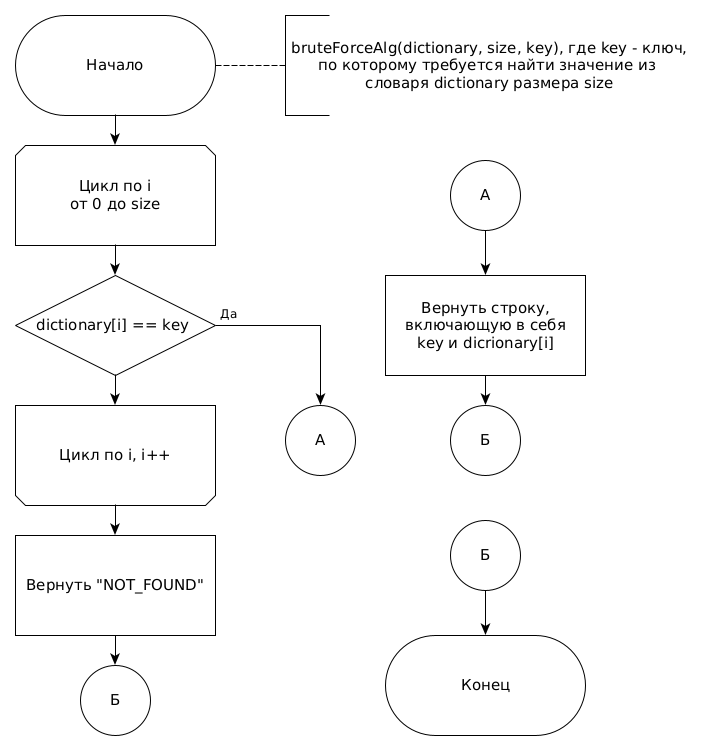
\includegraphics[scale=0.4]{inc/img/brutAlg.png}
\captionsetup{justification=centering}
	\caption{Схема алгоритма поиска полным перебором.}
	\label{img:brutAlg}	
\end{center}
\end{figure}

\newpage

\section{Схема алгоритма бинарного поиска по словарю}
Схема алгоритма бинарного поиска по словарю предоставлена на рисунке \ref{img:binAlg}.

\begin{figure}
\begin{center}
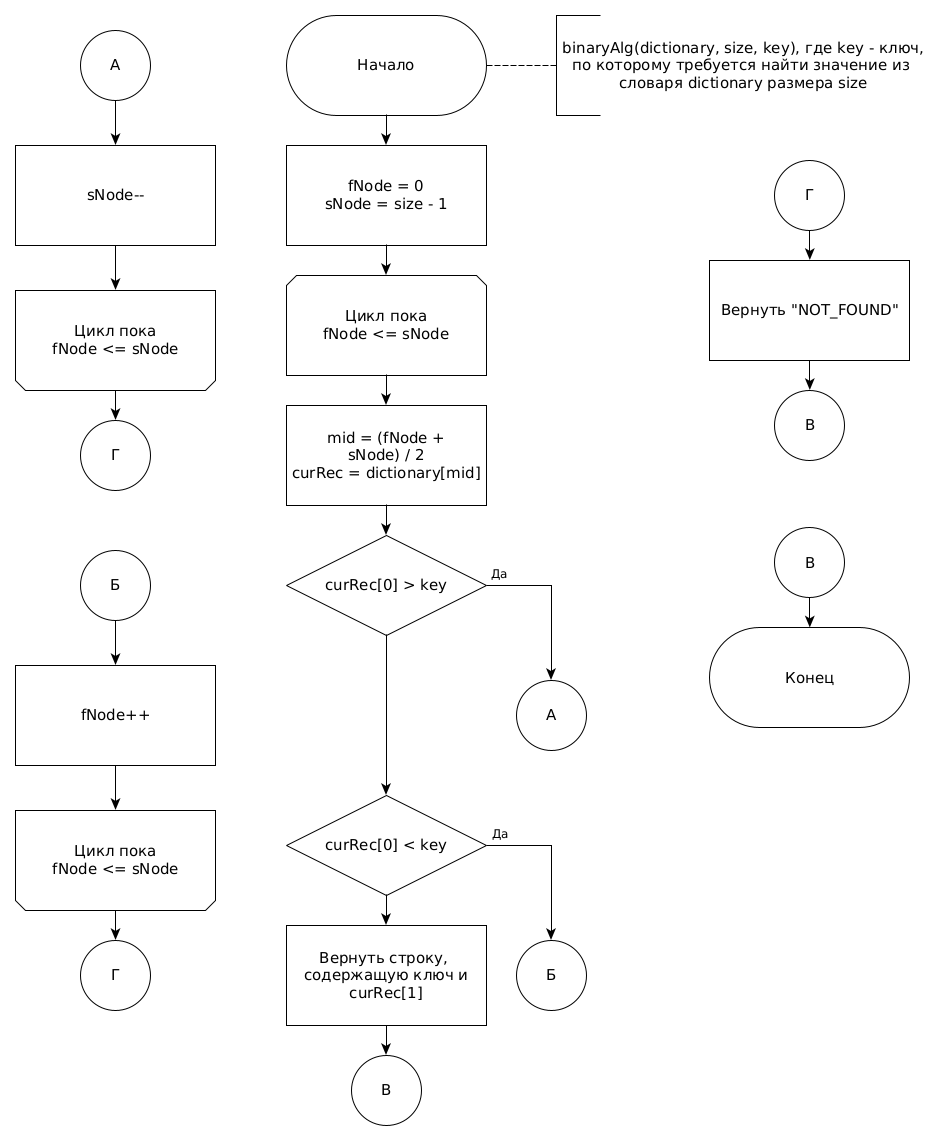
\includegraphics[scale=0.4]{inc/img/binAlg.png}
\captionsetup{justification=centering}
	\caption{Схема алгоритма бинарного поиска по словарю.}
	\label{img:brutAlg}	
\end{center}
\end{figure}

\newpage

\section*{Вывод}
Были представлены схемы алгоритма Брезенхема, а также реализации конвейерной обработки данных для данного алгоритма.

\chapter{Технологическая часть}
В данном разделе приведены требования к программному обеспечению, средства реализации программного обеспечения, а также листинг кода.

\section{Требования к программному обеспечению}
\begin{itemize}
\item входные данные - количество выполняемых задач (количество растеризуемых отрезков);
\item выходные данные - записи времени прихода и ухода обрабатываемых заявок для каждого реализованного конвейера.
\end{itemize}

\section{Средства реализации программного обеспечения}
При написании программного продукта был использован язык программирования C++ \cite{Cpp}.

Данный выбор обусловлен следующими факторами:
\begin{itemize}
\item данный язык программирования преподавался в рамках курса объектно-ориентированного программирования;
\item высокая вычислительная производительность;
\item большое количество справочной и учебной литературы в сети Интернет;
\item наличие реализации нативных потоков.
\end{itemize}

При написании программного продукта использовалась среда разработки QT Creator \cite{QT}.

Данный выбор обусловлен следующими факторами:
\begin{itemize}
\item основы работы с данной средой разработки преподавался в рамках курса программирования на Си;
\item QT Creator позволяет работать с расширением QtDesign, позволяющим создавать визуализируемый объект.
\end{itemize}

Для проведения замеров времени использовалась сторонняя библиотека Boost \cite{Boost}. Данная библиотека позволила фиксировать время прихода и ухода каждой заявки с точностью до наносекунд.

\section{Листинг кода}
В листингах \ref{list:bresAlg} и \ref{list:director} предоставлены реализации рассматриваемых алгоритмов.
\begin{lstlisting}[caption=Разбиение алгоритма Брезенхема,
label={list:bresAlg}]
std::string now_str()
{
    const boost::posix_time::ptime now = boost::posix_time::microsec_clock::local_time();

    const boost::posix_time::time_duration td = now.time_of_day();

    const long hours = td.hours();
    const long minutes = td.minutes();
    const long seconds = td.seconds();
    const long nanoseconds =
        td.total_nanoseconds() - ((hours * 3600 + minutes * 60 + seconds) * 1000000000);

    char buf[40];
    sprintf(buf, "%02ld:%02ld:%02ld.%09ld", hours, minutes, seconds, nanoseconds);

    return buf;
}

SegmentRasterizator::SegmentRasterizator(int xStart_, int yStart_, int xEnd_, int yEnd_)
{
    xStart = xStart_;
    yStart = yStart_;
    xEnd = xEnd_;
    yEnd = yEnd_;
    if (xStart == xEnd)
        xEnd += 1;
    else if (yStart == yEnd)
        yEnd += 1;

    image = new QImage(WIDTH, HEIGHT, QImage::Format_RGB32);
    image->fill(Qt::white);
}

int sign(float num)
{
    return (num < -__FLT_EPSILON__) ? -1 : ((num > __FLT_EPSILON__) ? 1 : 0);
}

void SegmentRasterizator::prepareConstantsForRB(int index)
{
    std::printf(ANSI_BLUE_BRIGHT "From START worker: task %d BEGIN %s" ANSI_RESET "\n", index, now_str().c_str());

    deltaX = xEnd - xStart;
    deltaY = yEnd - yStart;

    stepX = sign(deltaX);
    stepY = sign(deltaY);

    deltaX = std::abs(deltaX);
    deltaY = std::abs(deltaY);

    if (deltaX < deltaY)
    {
        std::swap(deltaX, deltaY);
        stepFlag = true;
    }
    else
        stepFlag = false;

    tngModule = deltaY / deltaX;
    mistake = tngModule - 0.5;

    std::printf(ANSI_BLUE_BRIGHT "From START worker: task %d ENDED %s" ANSI_RESET "\n", index, now_str().c_str());
}

void SegmentRasterizator::rastSegment(int index)
{
    std::printf(ANSI_MAGENTA_BRIGHT "From MIDDLE worker: task %d BEGIN %s" ANSI_RESET "\n", index, now_str().c_str());

    float curX = xStart, curY = yStart;
    for (int i = 0; i <= deltaX; i++)
    {
        dotsOfSegment.push_back(std::pair<int, int>(curX, curY));
        if (stepFlag)
        {
            if (mistake >= 0)
                (curX += stepX, mistake--);
            curY += stepY;
        }
        else
        {
            if (mistake >= 0)
                (curY += stepY, mistake--);
            curX += stepX;
        }
        mistake += tngModule;
    }

    std::printf(ANSI_MAGENTA_BRIGHT "From MIDDLE worker: task %d ENDED %s" ANSI_RESET "\n", index, now_str().c_str());
}

void SegmentRasterizator::createImg(int index)
{
    std::printf(ANSI_CYAN_BRIGHT"From END worker: task %d BEGIN %s" ANSI_RESET "\n", index, now_str().c_str());

    for (auto iter = dotsOfSegment.begin(); iter < dotsOfSegment.end(); iter++)
        image->setPixel(iter->first, iter->second, Qt::black);

    std::printf(ANSI_CYAN_BRIGHT "From END worker: task %d ENDED %s" ANSI_RESET "\n", index, now_str().c_str());
}

std::vector<std::pair<int, int>> SegmentRasterizator::getDotsOfSegment()
{
    return dotsOfSegment;
}
\end{lstlisting}

\begin{lstlisting}[caption=Менеджер потоков,
label={list:director}]
Director::Director(std::queue<SegmentRasterizator> &startQueue_)
{
    startQueue = startQueue_;
}

void Director::processPrepare()
{
    int i = 0;
    for (SegmentRasterizator curSeg(startQueue.front()); startQueue.size();
         startQueue.pop(), curSeg = startQueue.front())
    {

        curSeg.prepareConstantsForRB(i++);
        middleQueue.push(curSeg);
    }
}

void Director::processRast()
{
    int i = 0;
    while (startQueue.size() || middleQueue.size())
    {
        if (middleQueue.empty())
            continue;
        SegmentRasterizator curSeg(middleQueue.front());

        curSeg.rastSegment(i++);

		endQueue.push(curSeg);
        middleQueue.pop();
    }
}

void Director::processCreate()
{
    int i = 0;
    while (startQueue.size() || middleQueue.size() || endQueue.size())
    {
        if (endQueue.empty())
            continue;
        SegmentRasterizator curSeg(endQueue.front());

        curSeg.createImg(i++);
        endQueue.pop();
        final.push_back(curSeg);
    }
}

void Director::initWork()
{
    workers[0] = std::thread(&Director::processPrepare, this);
    workers[1] = std::thread(&Director::processRast, this);
    workers[2] = std::thread(&Director::processCreate, this);

    workers[0].join();
    workers[1].join();
    workers[2].join();
}

std::vector<SegmentRasterizator> Director::getFinal() { return final; }
\end{lstlisting}

\section{Тестирование программного продукта}
В таблице~\ref{tabular:test_rec} приведены тесты для функций, реализующих алгоритм Брезенхема. Тесты пройдены успешно.

\begin{table}[h!]
	\begin{center}
	
	\caption{\label{tabular:test_rec} Тестирование функций}
		\begin{tabular}{c@{\hspace{7mm}}c@{\hspace{7mm}}c@{\hspace{7mm}}c@{\hspace{7mm}}c@{\hspace{7mm}}c@{\hspace{7mm}}}
			\hline
			Точка начала отрезка (x, y) & Точка конца отрезка (x, y) & Ожидаемый результат \\ \hline
			\vspace{4mm}
			 (1, 1)&
			 (3, 3)&
			 (1, 1), (2, 2), (3, 3)\\
			\vspace{2mm}
			\vspace{2mm}
			 (1, 1)&
			 (1, 3)&
			 (1, 1), (1, 2), (1, 3)\\
			\vspace{2mm}
			\vspace{2mm}
			 (1, 1)&
			 (2, 1)&
			 (1, 1), (2, 1)\\
			\vspace{2mm}
			\vspace{2mm}
			 (3, 3)&
			 (1, 1)&
			 (1, 1), (2, 2), (3, 3)\\
		\end{tabular}
	\end{center}
\end{table}
\newpage

\section*{Вывод}
Спроектированные алгоритмы были реализованы и протестированы.

\chapter{Исследовательская часть}
\section{Технические характеристики}
Технические характеристики ЭВМ, на котором выполнялись исследования:
\begin{itemize}
\item ОС: Manjaro Linux 20.1.1 Mikah;
\item Оперативная память: 16 Гб;
\item Процессор: Intel Core i7-10510U.
\end{itemize}

При проведении замеров времени ноутбук был подключен к сети электропитания.

\section{Пример работы программного обеспечения}
На рисунке \ref{img:example} приведен пример работы программы для 7 визуализируемых отрезков.

\begin{figure}
\begin{center}
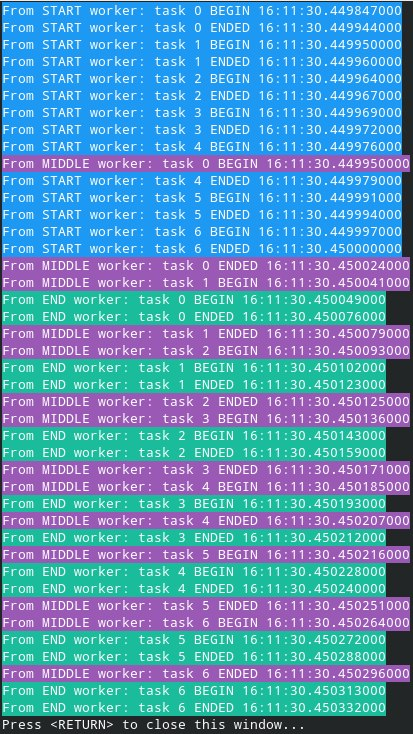
\includegraphics[scale=0.9]{inc/img/example.png}
\captionsetup{justification=centering}
	\caption{Пример работы ПО.}
	\label{img:example}	
\end{center}
\end{figure}

\newpage
\section{Время выполнения алгоритмов}
Алгоритм тестировался на данных, сгенерированных случайным образом.

В таблице \ref{time1} предоставлено время работы над каждым отрезком в предоставленном примере каждого из выделенных этапов.

Из таблицы видно, что среднее время выполнения этапа 1 составляет $\approx 17428.6$ наносекунд. Среднее время выполнения этапа 2 составляет $\approx 38285.7$ наносекунд. Среднее время выполнения этапа 3 составляет $\approx 18571.4$ наносекунд. Таким образом, этап 1 сравним по среднему времени выполнения с этапом 2. Но после выполнения этапа 1 заметно, что последующие вызовы функции работают за константное время, равное 3000 наносекунд, что при наличии начальных "прогревочных" запусков вылилось бы в факт того, что этап 1 не был бы сопоставим по среднему времени выполнения с этапом 3. Этап 2 является самым долго выполняющимся.

\begin{table}[h]
	\begin{center}
		\caption{\label{time1} Замеры времени для выполнения выделенных этапов.}
		\begin{tabular}{|c |c |c |c|} 
 			\hline
 			&\multicolumn{3}{|c|}{Время обработки, нс}\\
 			\hline
			Номер отрезка & Этап 1 & Этап 2 & Этап 3\\ [0.5ex] 
 			\hline\hline
 			0 & 97000 & 74000 & 27000 \\
 			\hline
 			1 & 10000 & 38000 & 21000 \\
 			\hline
			2 & 3000 & 32000 & 16000 \\
			\hline
			3 & 3000 & 35000 & 19000 \\
			\hline
			4 & 3000 & 22000 & 12000 \\
			\hline
			5 & 3000 & 35000 & 16000 \\
			\hline
			6 & 3000 & 32000 & 19000 \\
			\hline
			\end{tabular}
	\end{center}
\end{table}

\newpage

\section*{Вывод}
При сравнении результатов замеров по времени стало известно, что самым быстрым этапом конвейера оказался этап 1. При этом, самым медленным из трех рассмотренных - этап 2.

В среднем этап 1 работает быстрее этапа 2 на $\approx 20857.1$ наносекунд. При этом, при четвертой обработке отрезка разница в скорости выполнения составила 32000 наносекунд.

Этап 3 в среднем работает быстрее этапа 2 на $\approx 19714.3$ наносекунд. При этом, при шестой обработке отрезка разница в скорости выполнения составила 19000 наносекунд.

Таким образом, среднее время выполнения алгоритма для каждого отрезка составило $\approx 74285.71$ наносекунд.

\chapter*{Заключение}
\addcontentsline{toc}{chapter}{Заключение}
В ходе выполнения лабораторной работы была выполнена цель и следующие задачи:
\begin{enumerate}
\item[1)] было изучено асинхронное взаимодействие на примере конвейерной обработки данных;
\item[2)] была спроектирована система конвейерных вычислений;
\item[3)] была реализована система конвейерных вычислений;
\item[4)] была протестирована реализованная система;
\item[5)] был подготовлен отчёт по проведенной работе.
\end{enumerate}

Исследования показали, что в среднем:
\begin{enumerate}
\item[1)] этап 1 работает быстрее этапа 2 на $\approx 20857.1$ наносекунд;
\item[2)] этап 3 работает быстрее этапа 2 на $\approx 19714.3$ наносекунд;
\item[3)] среднее время выполнения алгоритма составило $\approx 74285.71$ наносекунд.
\end{enumerate}

\addcontentsline{toc}{chapter}{Литература}
\bibliographystyle{utf8gost705u}  % стилевой файл для оформления по ГОСТу
\bibliography{biblio.bib}          % имя библиографической базы (bib-файла)


\end{document} 
